Square $S_{1}$ is $1\times 1.$  For $i\ge 1,$ the lengths of the sides of square $S_{i+1}$ are half the lengths of the sides of square $S_{i},$ two adjacent sides of square $S_{i}$ are perpendicular bisectors of two adjacent sides of square $S_{i+1},$ and the other two sides of square $S_{i+1},$ are the perpendicular bisectors of two adjacent sides of square $S_{i+2}.$  The total area enclosed by at least one of $S_{1}, S_{2}, S_{3}, S_{4}, S_{5}$ can be written in the form $m/n,$ where $m$ and $n$ are relatively prime positive integers.  Find $m-n.$

\begin{center}
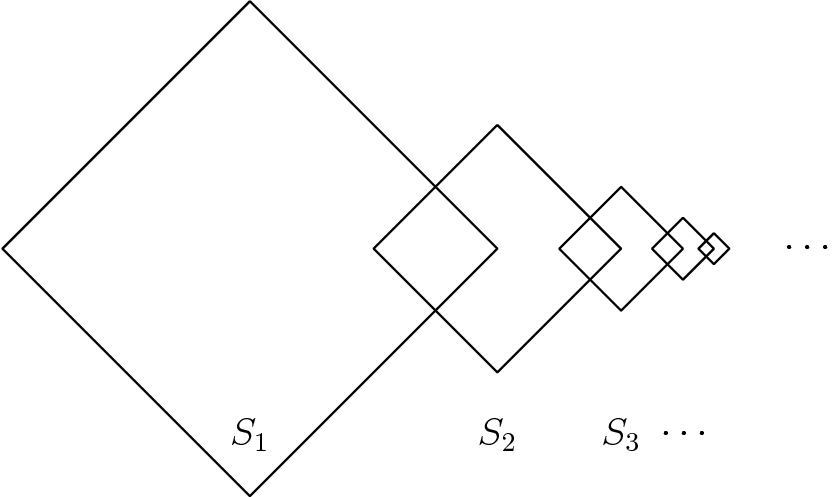
\includegraphics[width = 83.60000000000001mm]{img/fig0.png}
\end{center}